\newpage
\begin{song}{title={Nie mam dla ciebie miłości}, lyrics={Basia „Flow“ Adamczyk}, music={Skubas}, capo=1}
    \begin{intro}
        \writechord{C} \writechord{a7} \writechord{e(b6)} $\times 2$
    \end{intro}
    \begin{verse}
        ^{C}Jeśli chcesz, może^{Cmaj7}sz przyjść, kupi^{G6}ć wino, zosta^{a7}ć na noc \\
        ^{C}Nie przytulę cię ^{Cmaj7}potem, od^{G6}wrócę, rzucę \say{do^{a7}branoc} \smallskip \\
        Jeśli chcesz, możesz przyjść, zdjąć bluzkę, zostać do rana \\
        Nie odprowadzę cię potem, do drzwi trafisz sama
    \end{verse}
    \begin{chorus}
        ^{C}Nie mam dla ciebie mi^{a7}łości, ^{e} ktoś tu był przed ^{e7}tobą \\
        ^{C}Nie ma we mnie mi^{a7}łości, od^{e}chodząc zabrała ją ze ^{e7}sobą
    \end{chorus}
    \begin{verse}
        Jeśli chcesz, troszcz się o mnie, tylko pozbądź się złudzeń \\
        Nie zacznę cię kochać, choć przy tobie się budzę \smallskip \\
        Jeśli chcesz, to dbaj o mnie, bądź zawsze pod ręką \\
        Jeśli pójdę z inną, nie mów -- serce ci pękło
    \end{verse}
    \begin{chorus}
        Nie mam dla ciebie miłości, ktoś tu był przed tobą \\
        Nie ma we mnie miłości, odchodząc zabrała ją ze sobą \smallskip \\
        Nie mam dla ciebie miłości, ktoś tu był przed tobą \\
        Nie ma we mnie miłości, odchodząc\ldots
    \end{chorus}
    \begin{interlude}
        \writechord{C} \writechord{a7} \writechord{e} \writechord{e} $\times 4$ \\
        \writechord{e} \writechord{e}
    \end{interlude}
    \begin{outro}
        Nie mam dla ciebie miłości\ldots \smallskip \\
        Nie ma we mnie miłości\ldots $\times 2$
    \end{outro}
    \begin{center}
        \vfill{}
        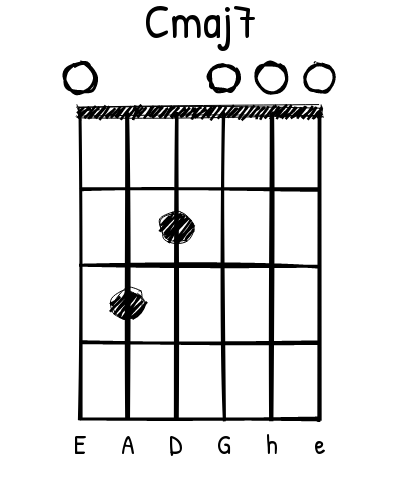
\includegraphics[height=3.5cm]{images/Cmaj7.png}
        \hspace{1cm}
        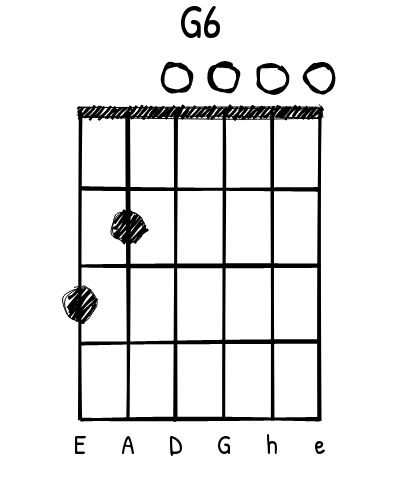
\includegraphics[height=3.5cm]{images/G6-easy.png}
        \vfill{}
    \end{center}
\end{song}

